\chapter{GALA: A Gamified Approach to Learning Algorithms}

%~ \centerline{{\LARGE\sl Exploring Basics of Algorithmic Approach}}
\vskip -12pt

\centerline{{\LARGE Exploring Basics of Algorithmic Approach}}

\vskip 0.8cm

\begin{center}
{\large\uppercase{$\text{Ram P. Rustagi}$}} 

\vskip -6pt

Department of CSE, KSIT Bengaluru

\end{center}

\vskip 1cm

\begin{center}
{\large\uppercase{$\text{Viraj Kumar}$}} 

\vskip -6pt

Divecha Centre for Climate Change, IISc Bengaluru

\end{center}


\vspace{2cm}

\centerline{\url{https://doi.org/10.34048/2021.1.F2}}

\vfill

%~ \begin{textblock}{16}(0,9)
%~ \noindent\centerimg[width=\paperwidth]{src/Figures/tcp.jpg}
%~ \end{textblock}


\newpage

\begin{multicols}{2}

\section*{Abstract}

In a typical Computer Science undergraduate programme, students take a two-course sequence in \textit{Data Structures and Algorithms} (DSA). These courses build on an introductory programming course which usually offers only a light introduction to these topics (e.g., the \textit{list} data structure implemented as an array, and simple algorithms such as \textit{linear search} and \textit{Bubble Sort}). Hence, the two-course DSA sequence is critical to help students to develop the skills necessary to create efficient algorithmic solutions to real-world problems. These skills are highly valued in industry, and the technical rounds in most job interviews evaluate these skills immediately after assessing the candidate's basic programming proficiency. Many students, particularly in institutions outside the top tier, fail to clear these hurdles because they have not been given enough opportunity to hone these skills. In this series of articles, we describe a new approach to address these shortcomings - a Gamified Approach to Learning Algorithms (GALA). We describe our approach in the context of the Algorithms course (typically the second in the 2-course DSA sequence). Student feedback (drawn from an institution outside the top tier) confirms that this approach enables students to grasp key concepts, and to develop a better understanding of how and why the algorithm works. Following the introduction of GALA, we are also starting to see improved student performance on job interviews.

\vspace{-.3cm}

\section{Introduction}\label{section-1}

\vspace{-.2cm}

A recent report by Aspiring Minds \cite{art2-key01} estimates that more than 90\% of graduating engineers ``do not have the desired programming and algorithm skills required to work in IT product companies". Such companies expect graduates to have the ability to create an algorithmic solution to a real-world problem (and then implement this solution in code). The former task involves at least three key skills: \textit{modeling} the concrete problem in abstract terms, \textit{recognizing} opportunities (if any) to reduce this problem to one for which an efficient algorithm (using appropriate data structures) already exists, and (when necessary) \textit{developing} an algorithm to solve this problem as efficiently as possible. Note that each of the three action verbs associated with these tasks (\textit{modeling, recognizing}, and \textit{developing}) are at the higher levels of Bloom's Taxonomy. However, in many of the Data Structures and Algorithms (DSA) courses we have reviewed at institutions outside the top-tier, the emphasis is on tasks at the two lowest level of Bloom's Taxonomy: Remembering (e.g., \textit{memorizing} an algorithm or the detailed implementation of a particular data structure) and Understanding (e.g., \textit{tracing} an algorithm's behaviour on a given input, or tracing the evolution of a data structure on a given sequence of operations). As the Aspiring Minds report \cite{art2-key01} indicates, such courses do not prepare graduates adequately for industry needs.

This series of articles describes a pedagogical approach to teaching an \textit{Algorithms} course that meets two simultaneous objectives:

\vspace{-.2cm}

\begin{itemize}  
\item[$\bullet$] Objective 1: It hones the three key skills noted above.\\[-.4cm]
\item[$\bullet$] Objective 2: It is workable in institutions outside the top-tier.\\[-.4cm]
\end{itemize}
  
\vspace{-.2cm}  
  
Institutions outside the top-tier lack many of the advantages that top-tier institutions possess. For instance, many of their students have limited language proficiency, analytical reasoning, and mathematical maturity. Further, almost no course prior to their \textit{Algorithms} course hones their higher-order thinking abilities. (Even the introductory programming course tends to be syntax-heavy, and focused on skills at the two lowest levels of Bloom’s Taxonomy.) As an illustration, consider the \textit{Algorithms} course taught by the first author. In the preceding introductory programming course, almost all students were able to correctly reproduce the \textit{Bubble Sort} algorithm when asked. The first author reminded students of the \textit{Bubble Sort} algorithm, and then asked them to use it to sort the university roll numbers of 10 students. About 80\% of the class was unable to apply this algorithm to the given data (a task that is no higher than level 3 of Bloom’s Taxonomy). In the same institution, when the first author asked senior students to analyze the time complexity of the algorithm(s) implemented in their final-year project, the vast majority of students were unable to apply these skills to the given task. Such a context requires an approach that students find initially \textit{accessible} yet sufficiently \textit{engaging} that they are motivated to spend enough time grappling with the problem. (Tasks associated with higher levels of Bloom's Taxonomy require students to spend time evaluating multiple possible ways of tackling them.)  
 
\vspace{-.3cm}   
 
\section{GALA: Accessible and Engaging}\label{section-2}  
  
\vspace{-.2cm} 
  
Our Gamified Approach to Learning Algorithms (GALA) is designed to be both accessible and engaging. We assume a lecture of between 40 and 60 minutes, and we split this into two approximately equal parts. In Part 1 (20 to 30 minutes), students play a game that, by its design, requires interactive engagement to develop an algorithm. We ensure accessibility in two ways. First, the rules are specified using language that is as simple and unambiguous as possible. Second, wherever possible, students play the game with physical artefacts. As we shall explain, these can be created easily and inexpensively. In Part 2 (the remaining 20 to 30 minutes), the instructor explains one or more efficient algorithm to solve the problem, leveraging the students’ familiarity with and interest in the problem developed in Part 1. In many cases, the games themselves are well-known. Our contribution lies in weaving these games into a pedagogy to support desired learning outcomes in the \textit{Algorithms} course.  
  
In-class observations confirm that students find the games accessible and deeply engaging. Further, the feedback collected from our students confirms that GALA enables students to grasp key concepts, and to develop a better understanding of how and why certain algorithms work. Following the introduction of GALA, we are also starting to see improved student performance on job interviews. In the next three sections, we illustrate GALA through examples.

\vspace{-.3cm}

\section{Game 1: Decimal to Binary}\label{section-3}  

\vspace{-.2cm}

The purpose of this game is to help students understand the classical algorithm for converting positive integers from decimal to binary representation (Table~\ref{chapter3-table-1}) at a deeper level than a mere sequence of steps. One way to achieve this is through a formal (inductive) proof of correctness.
  
As we have noted above, we cannot assume that students will have the requisite mathematical maturity to fully understand (let alone develop) such a proof. Hence, the game aims to help students understand the ``core" of such a proof, without using the language of induction. More importantly, the game gives students an opportunity to hone their skills in \textit{developing} algorithms. 
\begin{table}[H]
\vspace{-.3cm}
\centering
\caption{Algorithm for converting decimal to binary}\label{chapter3-table-1}
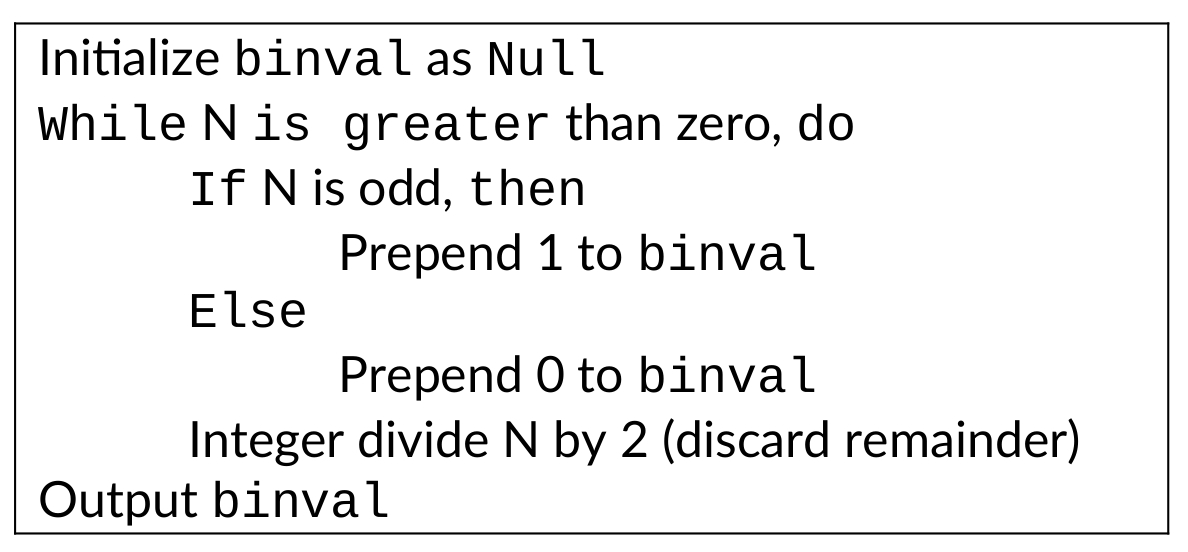
\includegraphics[scale=.9]{src/Figures/chap2/table1.jpg}

\vspace{-.5cm}

\end{table}

There are several versions of this game, and we first describe the rules of the simplest version (Version 1). All versions of this game are played with two players: $P_{1}$ and $P_{2}$. Player $P_{1}$ has a set of 7 cards numbered $C_{1}, C_{2},..., C_{7}$, each with 64 numbers (Table~\ref{chapter-3-table-2}). Player $P_{2}$ begins the game by guessing a number $N$ between 1 and 127 (both inclusive) without revealing it to $P_{1}$. Next, for each card $C_{1}, C_{2}, ..., C_{7}$, $P_{1}$ asks $P_{2}$ whether $N$ appears on this card. For each question, $P_{1}$ notes $P_{2}$'s response (yes/no). Note that $P_{2}$ must never lie! (If $P_{2}$ lies, at the end of game, $P_{1}$ can easily prove that $P_{2}$ lied). At the end, $P_{1}$ must correctly identify the number that $P_{2}$ had guessed based on the set of yes/no response for each card $C_{i}$. 
  
While a ``brute force" approach is possible by carefully ruling out all numbers except one, this is clearly a tedious process. Students quickly realize that they need to come up with some clever ``formula" (i.e., an algorithm!) to combine the yes/no answers into a single number that $P_{2}$ has guessed.  
%~ \end{multicols}

\begin{table}[H]

\vspace{-.3cm}

\centering
\caption{A set of 7 cards for Version 1}\label{chapter-3-table-2}
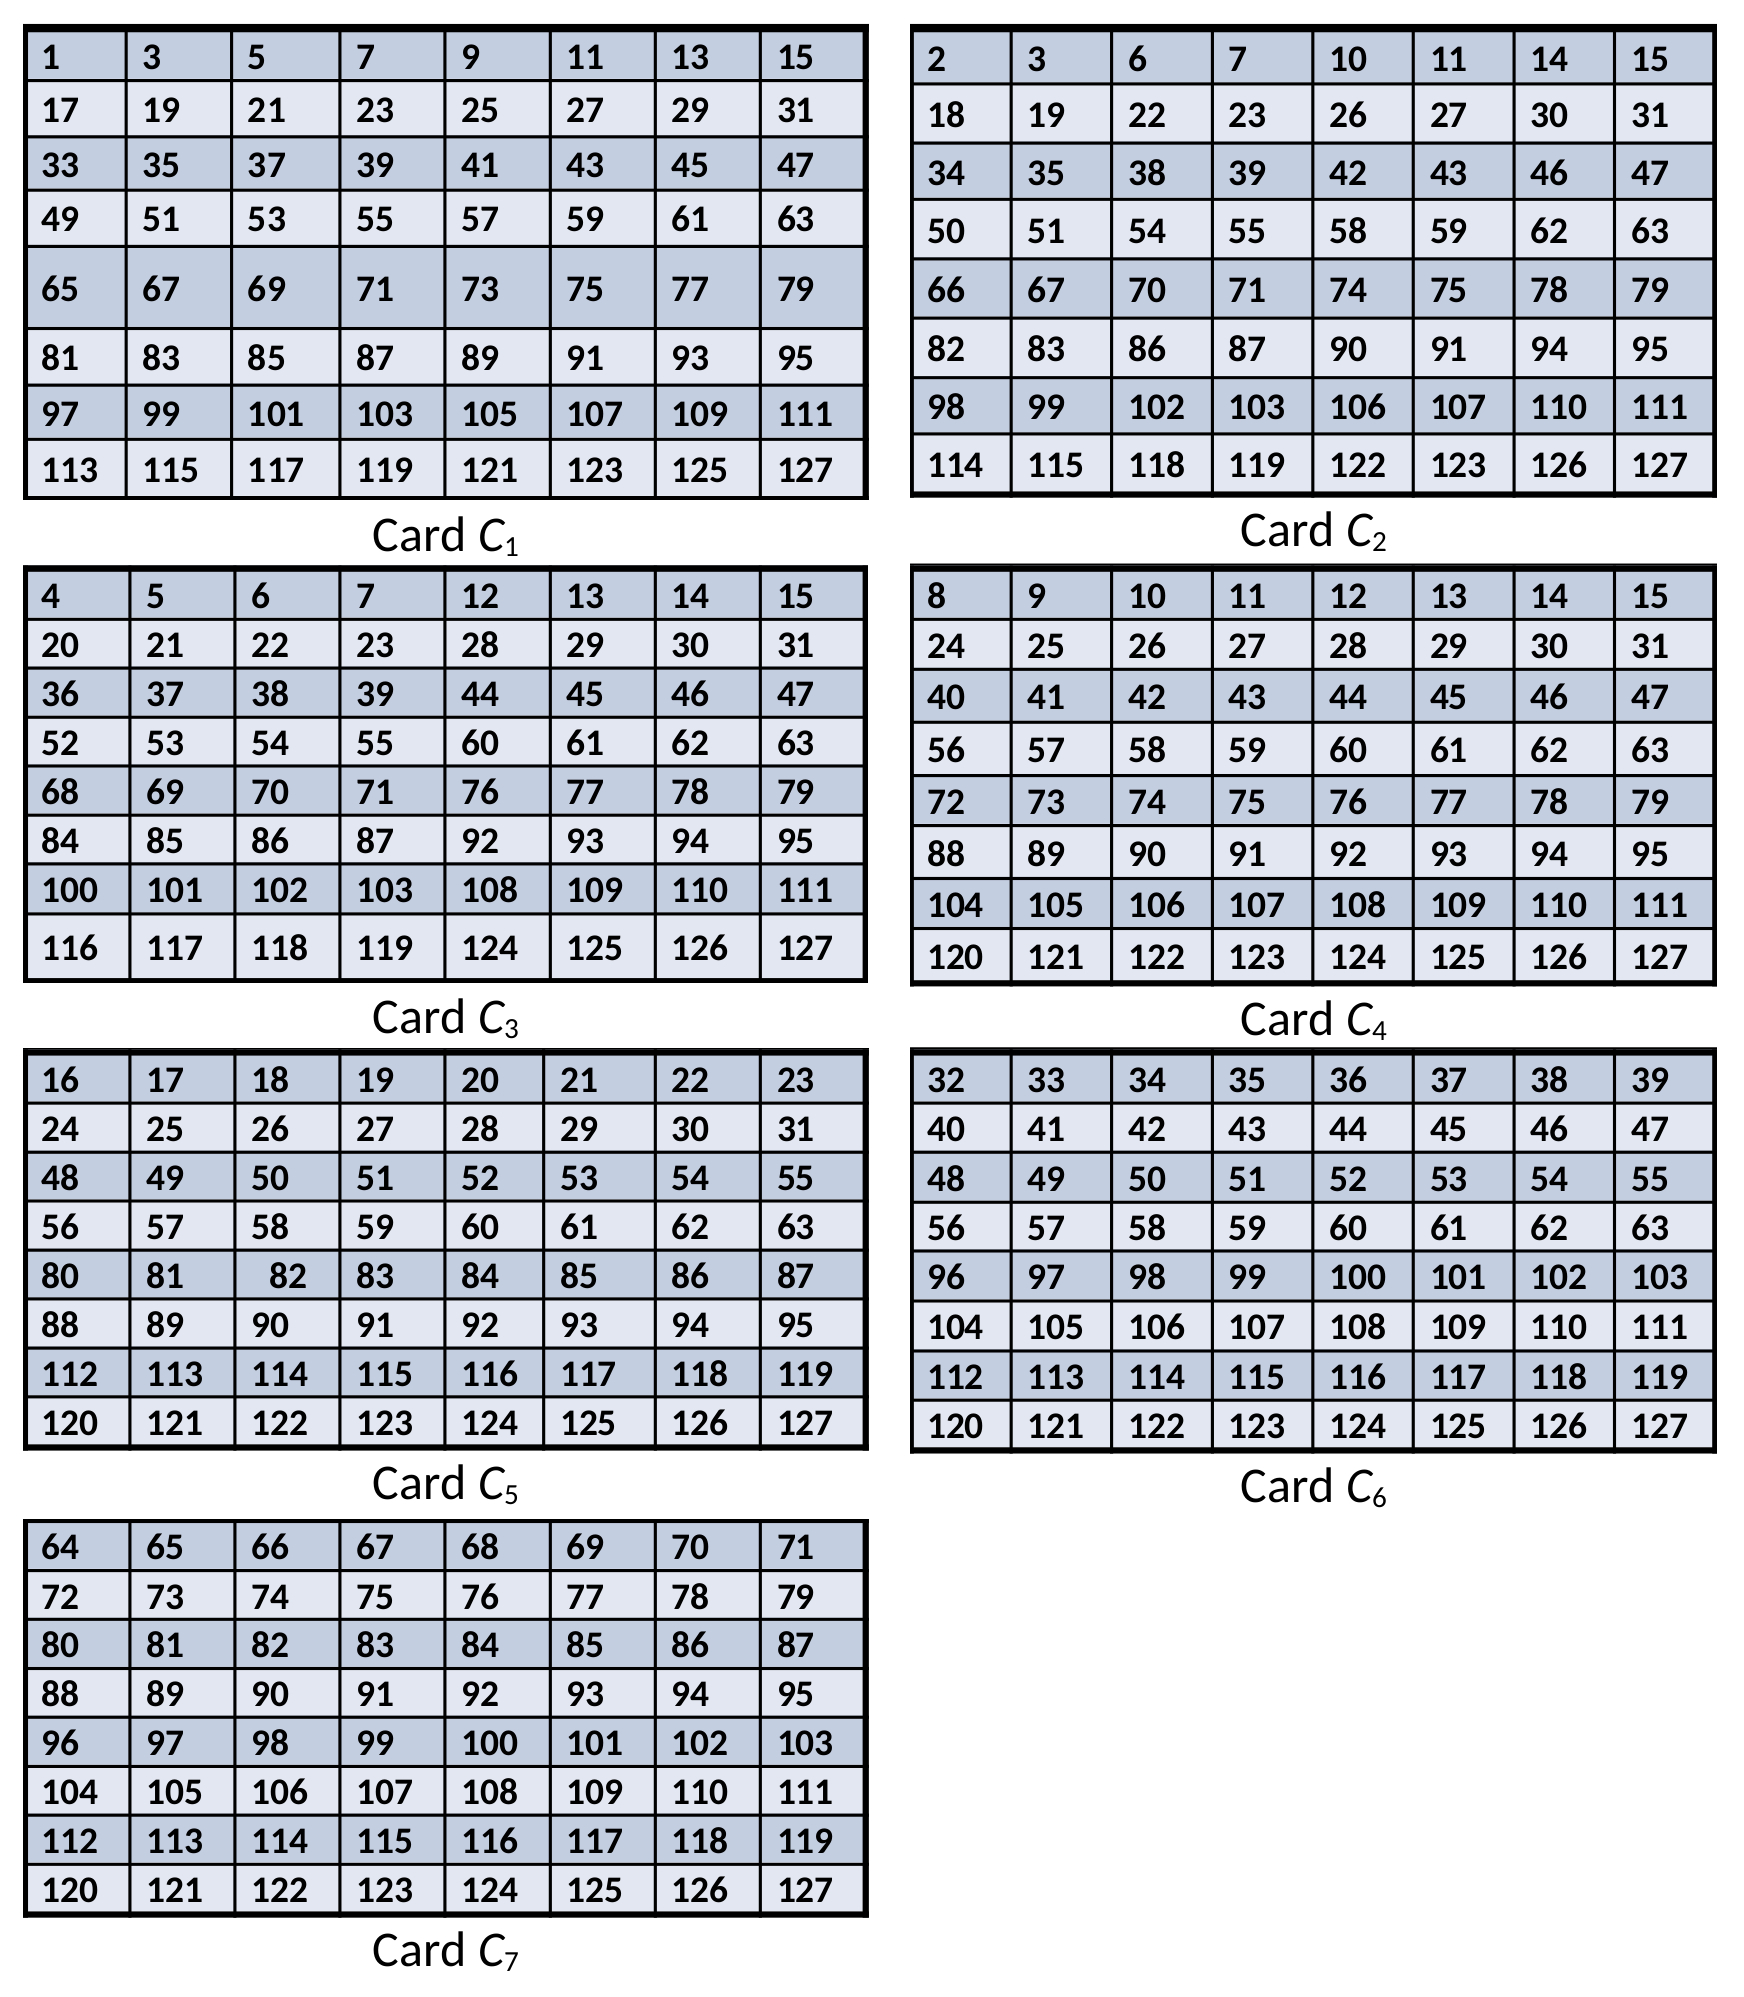
\includegraphics[scale=.62]{src/Figures/chap2/table2.jpg}
\end{table} 

\vspace{-.7cm}

%~ \begin{multicols}{2}
We split the class into groups of 4, and we give each group a full set of 7 cards. (An entire set can be printed on a single A4 sheet of paper and easily cut out.) Each member of the group is asked to take turns playing the role of $P_{2}$, while the rest of the group plays the role of $P_{1}$. Before proceeding further, we encourage you to pause and try the game! For example, if we play the role of $P_{2}$ and tell you that our number appears only on cards $C_{1}, C_{2}, C_{6}$ and $C_{7}$, can you identify our number?


When students in a class of about 60 students (15 groups) were allowed to play this game for 15-20 minutes, only two groups were able to correctly identify an algorithm to compute the guessed number. However, neither of these groups was able to explain \textit{why} their algorithm worked. Even with this limited success, each group had their ``Aha!" moments. Finally, when the logic and the underlying theory was explained (in Part 2), almost the entire class was thrilled. We will now discuss the concepts involved and why the logic works.

To compute the guessed number, we should sum up the values $2^{i-1}$ for each card $C_{i}$ for which $P_{2}$ answers yes. For our example above (yes to $C_{1}, C_{2}, C_{6}$ and $C_{7}$), the sum is $2^{0} + 2^{1} + 2^{5} + 2^{6} = 99$. You can confirm that 99 is the only number that appears on precisely this set of four cards. 
 
To understand why the logic works, we should refresh the theory of number representation using the underlying number base and place value of digits. For example, the decimal number 4763 corresponds to $4\times10^{3}+7\times10^{2}+6\times10^{1}+3\times10^{0}$. The position of the digit in the number has its corresponding place value, determined by respective power of 10 (decimal base value). Thus, in a 4-digit decimal number, place values are defined corresponding to unit place, tenth place, hundredth place and thousandth place value. The digit in each position is to be multiplied with its position-based place value and when all the values are summed, we get the number.  When the number is represented in binary, the base value is taken as 2. When a number is represented using 7 binary digits, the value $N$ is computed as $N=x_{7}2^{6}+x_{6}2^{5}+x_{5}2^{4}+x_{4}2^{3} + x_{3}2^{2}+x_{2}2^{1} + x_{1}2^{0}$, where $x_{i}$ corresponds to the $i^{\rm th}$ binary digit. The decimal number 99 in binary is written as 1100011. In this binary representation, digits $x_{1},  x_{2}, x_{6}$ and $4x_{7}$ are 1, and remaining 3 binary digits $x_{3}, x_{4}$ and $x_{5}$ are zero. Thus, the value would be computed as $1\times2^{6} + 1\times 2^{5} + 0\times 2^{4} + 0\times 2^{3}+0\times 2^{2}+1\times 2^{1} +1\times 2^{0} = 2^{6} + 2^{5} + 2^{1} + 2^{0} = 64 + 32 + 2 + 1 = 99$. 

A closer analysis of card $C_{i}$ reveals that the first number is precisely $2^{i-1}$. More interestingly, every number on card $C_{i}$ contains $2^{i-1}$ in its binary expansion. Thus, whenever player $P_{2}$ responds to a card $C_{i}$, player $P_{1}$ learns the $i^{th}$ bit of $N$ (yes means 1, no means 0). While this is clearly not a formal proof of correctness, understanding this key point helps students better understand why the algorithm in Table~\ref{chapter3-table-1} works: each iteration $i$ of the loop is evaluating the $i^{th}$ bit of $N$. Of course, we can present this as a dry fact to students, and they could certainly reproduce this fact on an exam. Instead, GALA provides a much deeper learning experience: students quickly realize that there is \textit{some} pattern to the numbers, and they immediately engage with trying to discover this pattern. The ability of a student to recognize patterns (or more abstractly, ``properties") is critical to their ability to develop algorithms, since algorithms exploit these patterns/properties.
 
To further hone this skill, a variant of the same game can be played (Version 2) using a different set of cards $C’_{1}, C’_{2},..., C’_{7}$ (Table~\ref{chapter-3-table-3}). In this variant, the logic is reversed: a ``yes" to card $C’_{i}$ means that the $i^{th}$ bit of $N$ is $0$ (“no” means the bit is 1). Several other variations of the game can be played by mixing cards from these two sets – care must be taken to map yes/no answers for the two types of cards ($C_{i}$ and $C’_{i}$) to 1/0 bits. Cards can be printed in different colours (blue vs. orange), or students can recognize that all cards of type $C’_{i}$ start with the number 0. Another variant could be to use a set of 5, 6 (or N) cards instead of 7, in which case count of numbers appearing on each card would change accordingly. For example, for a set of 5 cards, each card would have 16 numbers and so on. 
 
\begin{table}[H]

\vspace{-.3cm}

\centering
\caption{A set of 7 cards for Version 2}\label{chapter-3-table-3}
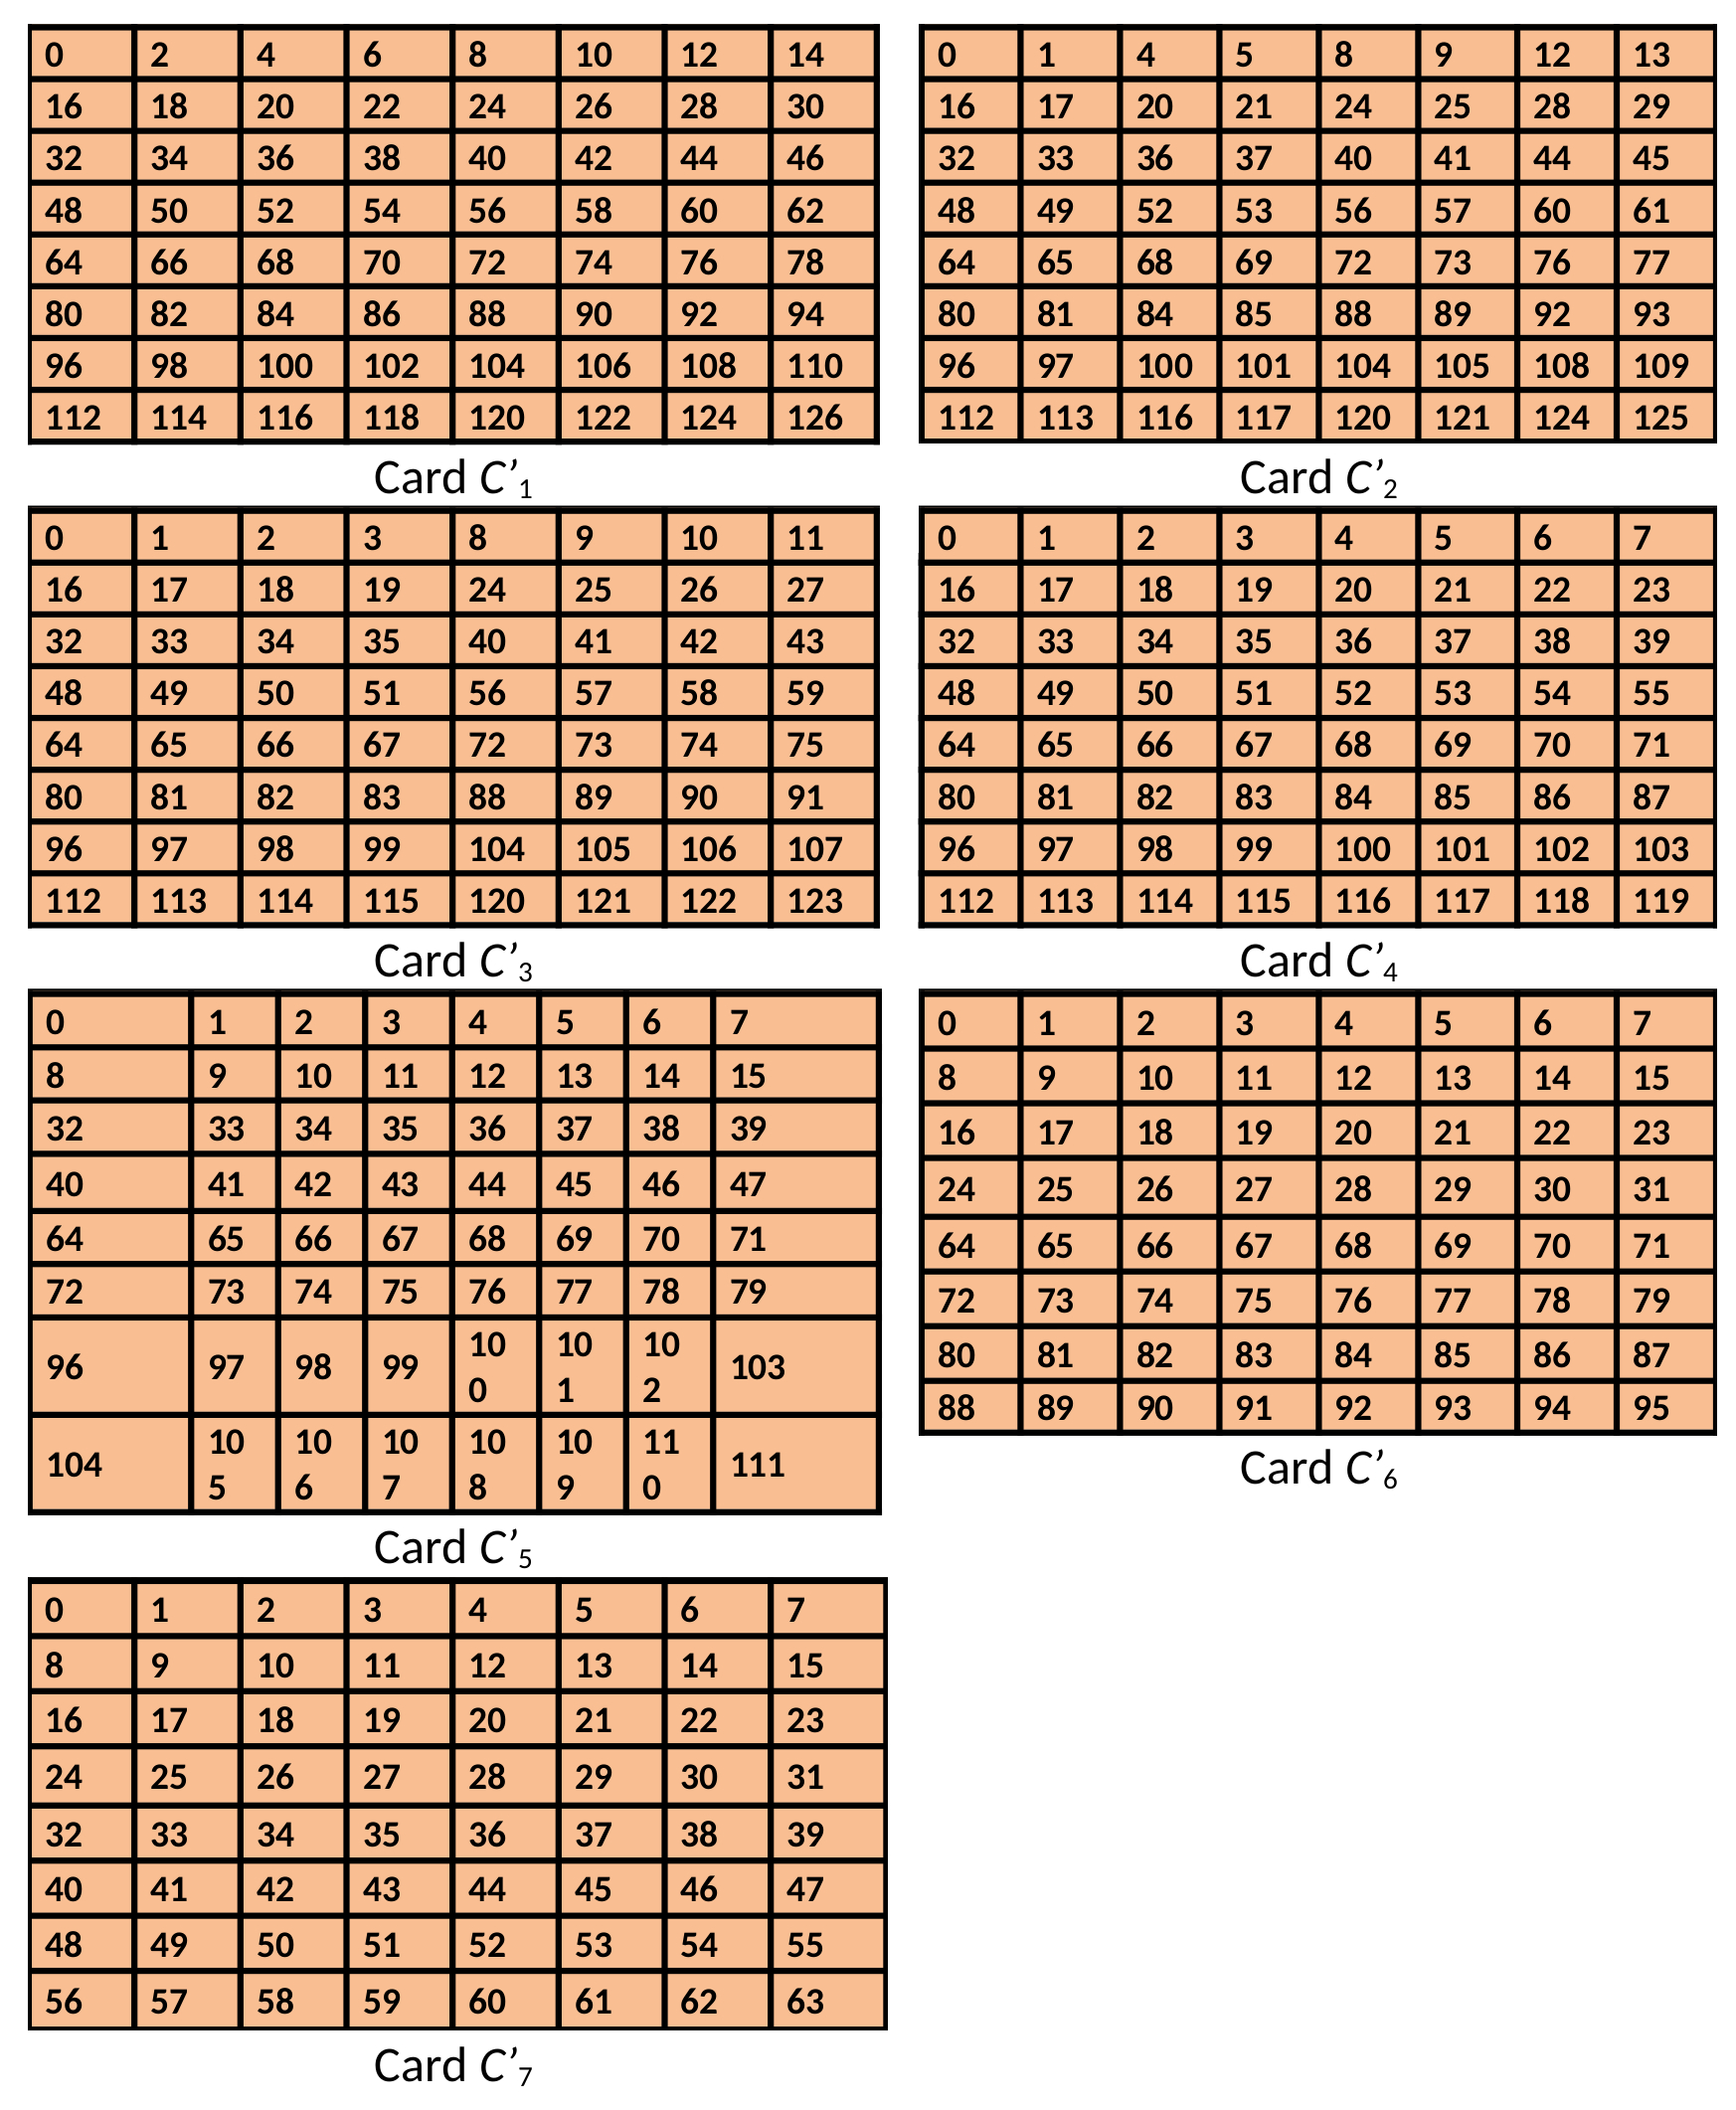
\includegraphics[scale=.62]{src/Figures/chap2/table3.jpg}

\vspace{-.3cm}

\end{table}

\vspace{-.3cm}

\section{Game 2: Euclid's Game}\label{section-4} 

\vspace{-.2cm}

Next, we discuss a classic game known as Euclid’s game \cite{art2-key02}\cite{art2-key03}. Once again, our purpose is to use this game to hone student's abilities to develop algorithms. This 2-player game requires nothing more than a sheet of paper and a pen. Player $P_{1}$ writes down two unequal positive numbers, and player $P_{2}$ must decide whether to make the first move or the second move. Thereafter, the two players make alternate moves as decided by $P_{2}$. In each move, a player must write a positive number $x$ that satisfies two properties:
\begin{itemize}

\item[\bullet] $x$ must be the difference of two numbers already on the paper, and

\item[\bullet] $x$ must not appear previously on the paper
\end{itemize} 

The first player who cannot write such a number $x$ loses the game. The algorithmic task for students is to determine a winning strategy for $P_{2}$. In other words, students must write an algorithm whose inputs are two distinct positive integers $m$ and $n$ (the numbers written by $P_{1}$), and whose output is 1 if $P_{2}$ should make the first move, or 2 if $P_{2}$ should make the second move.

We split the class into groups of 4, and we work out an example such as the following. Suppose $P_{1}$ writes $m = 25$ and $n = 35$, and suppose $P_{2}$ decides to make the \textit{second} move. Then the game could proceed as follows:
\begin{itemize}
\item[i.] $P_{1}$ writes 10 (this is the only valid number that can be written)
\item[ii.] $P_{2}$ writes 15 (the difference of 25 and 10). Note that $P_{2}$ cannot write 25 (the difference of 35 and 10), since that has already been written.
\item[iii.] $P_{1}$ writes 20 (the difference of 35 and 15). At this stage, $P_{1}$ could have also written 5 (the difference of 15 and 10).
\item[iv.] $P_{2}$ writes 5 (the difference of 25 and 20).
\item[v.] $P_{1}$ writes 30 (the difference of 35 and 5).
\end{itemize}

At this point, $P_{2}$ loses because no new number can be written. We now split students into groups of about 4 and allow them 10 minutes to come up with a winning strategy for $P_{2}$. Most groups start (sensibly) by playing the game with the same numbers $m$ and $n$, but with $P_{2}$ making the first move. These groups are often able to convince themselves that no matter what numbers $P_{1}$ writes, $P_{2}$ can win the game. In fact, these groups recognize that no matter what choices the players make, the same numbers 5, 10, 15, 20, 25, 30 are written down when $m = 25$ and $n = 35$. At this point, we observe many groups proposing incorrect or incomplete algorithms. For instance, some groups surmise that $P_{2}$ should make the first move when both numbers are odd and the second move when both numbers are even. We then provide counter-examples such as $m = 30$ and $n = 70$ where $P_{2}$ must make the first move in order to win, and $m = 25$ and $n = 40$ to point out cases that students have not considered.


These counter-examples make the problem more interesting, and students continue to look for patterns in the games. Given enough time, most groups realize that the set of all numbers written on the paper (including $m$ and $n$) can \underline{always} be sorted to produce numbers of the form: $a, 2a, ..., min(m, n), ..., max(m, n)$. Since all these numbers are multiples of $a$, it becomes clear that a is a common factor of both $m$ and $n$. A handful of groups realize that the number a must be the highest such common factor (also called the greatest common divisor or GCD) of $m$ and $n$. Even groups that fail to grasp this insight on their own are able to recognize its truth when we present it to them. From this point, their task is to merely recognize that if $max(m, n) = k \times a$, then $P_{2}$ should go first if $k$ is odd, and $P_{2}$ should go second otherwise.

It is useful to reflect for a few minutes on why this strategy is correct. There are $k$ numbers that can be written: $a, 2a, …, k \times a$. Since two of these numbers are $m$ and $n$, the players can only write the remaining $k - 2$ numbers. Hence, $P_{2}$ can guarantee a win by going first when $k - 2$ is odd (which implies that $k$ is odd) and going second when $k - 2$ is even.

\vspace{-.3cm}

\section{Game 3: Pouring Milk}\label{section-5}

\vspace{-.2cm}

Finally, we describe a game that can hone student's abilities to abstractly model a simple real-life problem and also recognize the similarities between this problem and one already solved. We ask students to consider a vendor who sells milk from a large tanker. The vendor extracts milk using one of two jugs, one with capacity $m$ liters and \underline{another} with capacity $n$ liters, where $m$ and $n$ are distinct positive integers. (Attentive students and the reader might start seeing connections with the previous game already!) The jugs have no intermediate markings, so the only known volumes of milk the vendor can directly measure is by filling a jug to capacity ($m$ liters or $n$ liters). We ask students to design an algorithm to give a customer exactly $k$ liters of milk using the two jugs, or to report that this is impossible. Note that $k$ must also be a positive integer.

As an example, see if you can find a solution when\break $m = 5, n = 7$, and $k = 1$. When we present this problem to students, some of them indicate that they have seen similar puzzles before, but usually with specific numbers only (not in the general form with numbers $m, n,$ and $k$). Although this is not a 2-player (or multi-player) game, we once again ask students to work in groups with about 4 members each. Most groups, especially those in which a student has seen this type of puzzle before, quickly realize that the vendor can measure some volumes (other than $m$ and $n$) by pouring milk from one jug to the other. Specifically, if the vendor fills the 7-liter jug to capacity from the tank, then pours the milk from this jug into the 5-liter jug until it reaches capacity, then the 7-liter jug now contains precisely 2 liters of milk. At this point, some groups recognize that the vendor has computed the difference (7 – 5 = 2) of the given numbers $m = 5$ and $n = 7$, and they sense there are similarities with Game 2.

Indeed, it is possible to precisely measure only those volumes k that are multiples of the GCD of $m$ and $n$. In the above example, the GCD of 5 and 7 is 1, and hence it is possible to measure out 1 liter. Algorithm to compute GCD of two numbers using repeated subtraction is given in Table~\ref{chapter-3-table-5} (Appendix) and its optimized version using remainder operation is given in Table~\ref{chapter-3-table-6}. To find a sequence of steps, students must create an appropriate \textit{abstract model} to represent the current volume of milk in the two jugs as they pour milk in and out of them. The simplest mathematical representation is a tuple \textit{(p, q)}, where \textit{p} represents the volume of milk in the jug with capacity $m$ $(0 \leq p \leq m)$, and $q$ represents the volume of milk in the jug with capacity $n$ $(0 \leq q \leq n)$. Students with weak mathematical maturity may not use such a concise notation, but we do observe many groups developing similar notation. We present the tuple notation when we discuss our approach in Part 2 of this exercise.

In this notation, the vendor starts with the tuple\break (0, 0) representing the situation where both jugs are initially empty. We now describe a sequence of steps the vendor can perform to measure 1 liter of milk for the customer. The sequence starts with these four steps:\break (0, 0)$\rightarrow$(5, 0)$\rightarrow$(0, 5)$\rightarrow$(5, 5)$\rightarrow$(3, 7). Thus, starting with both jugs empty, we first fill the 5-liter jug to capacity (step 1), leading to the tuple (5, 0). Then, (step 2) we transfer this milk to the 7-liter jug (0, 5), then (step 3) we again fill the 5-liter jug to capacity (5, 5). Lastly (step 4), we transfer milk from the 5-liter jug to the 7-liter jug until it reaches capacity. At this point, 2 liters of milk have been transferred, leading to the tuple (3, 7). The remaining steps are: (3, 7) $\rightarrow$ (3, 0)  (0, 3) $\rightarrow$ (5, 3) $\rightarrow$ (1, 7). (Note that we go from (3, 7) to (3, 0) by emptying all the milk in the 7-liter jug back into the milk tanker!) At this point, the 5-liter jug contains precisely 1 liter of milk, as desired by the customer.

By allowing students enough time (about 20 minutes) to experiment with several examples, a few groups realize that they can ``make progress" (i.e., measure new volumes of milk) using a systematic process which lies at the heart of the solution (i.e., the while-loop) shown in Table~\ref{chapter-3-table-4}. Note that we are assuming that $m < n$. We leave it as an exercise for you to see if the same algorithm also works when $n < m$.

\begin{table}[H]

\vspace{-.3cm}

\centering
\caption{Algorithm for Game 3}\label{chapter-3-table-4}
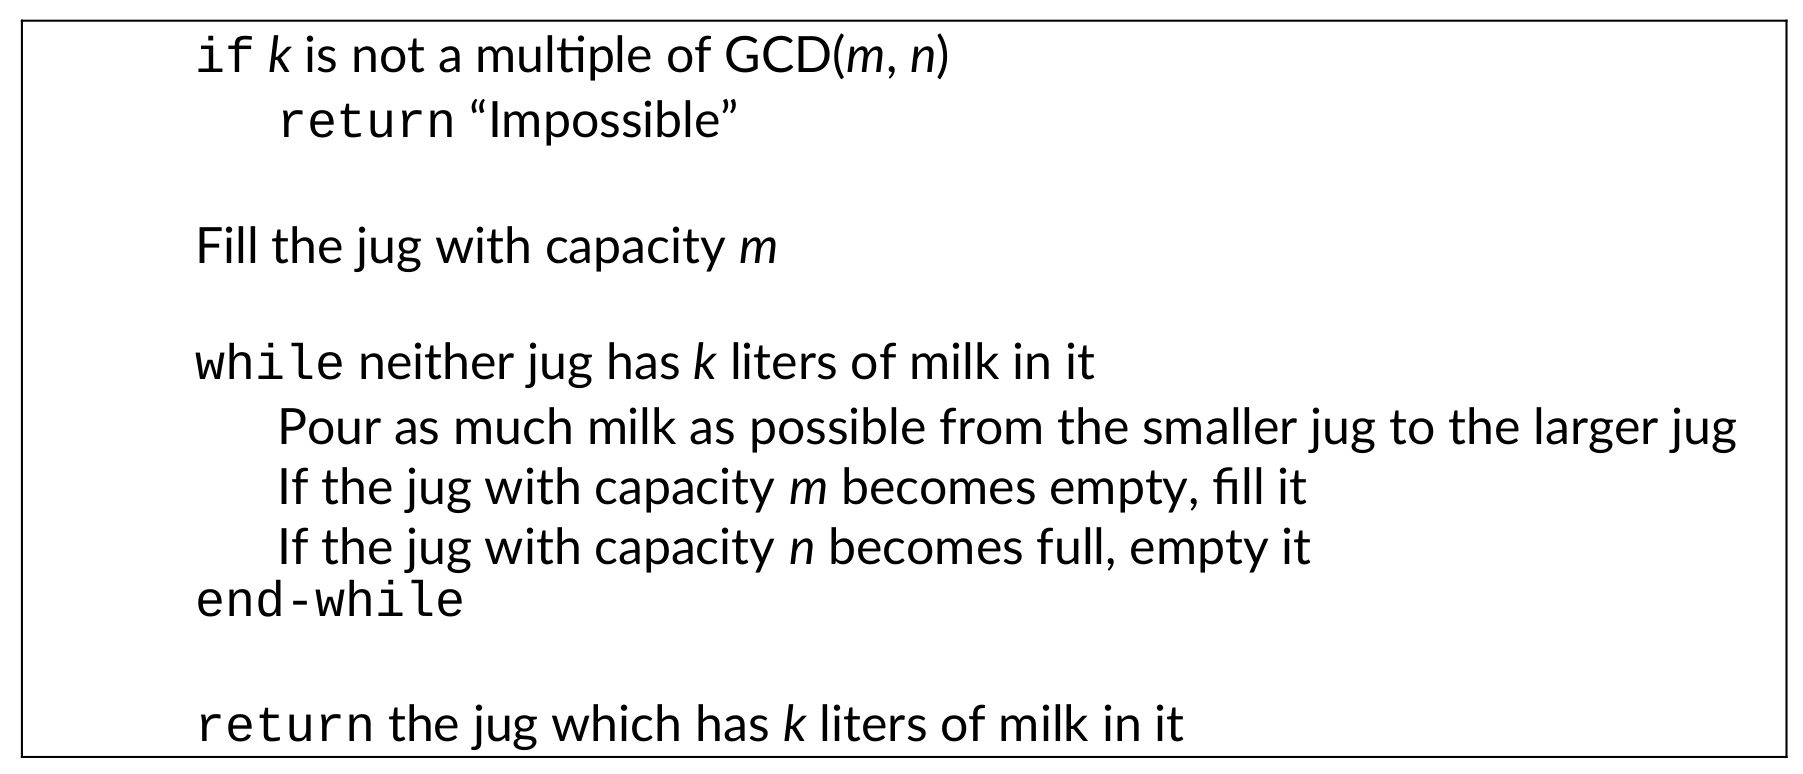
\includegraphics[scale=.6]{src/Figures/chap2/table4.jpg}
\end{table}

\vspace{-.5cm}

When we discuss our approach, we work out several examples using the tuple notation to help students model the problem and start seeing the pattern. We also point out the similarities between Games 2 and 3. By pouring milk from one jug to another (Game 3), we are essentially computing the same differences that we saw in Game 2. Although this idea can be made more precise, we do not delve into these connections here. In a later article, we will present examples of games where we highlight the connection between two games to demonstrate the powerful idea of reduction.

\vspace{-.3cm}

\section{Summary}

\vspace{-.2cm}

We have found the GALA approach effective in maintaining student engagement in classes of more than 50 students, both during the initial game-play (Part 1) and during the subsequent explanations (Part 2). Student feedback on this approach is consistently positive, and students demonstrate greater confidence in attacking algorithmic design challenges.

As an instructor, you may wonder whether this approach can be applied to ``all algorithms in the syllabus". We have found that GALA is useful for only a few algorithms, so it cannot be applied wholesale for all topics in a typical \textit{Algorithms} course. Nevertheless, as we will demonstrate over the next few articles, it can be used to enhance student learning for several interesting algorithms.

\section{Appendix}

\begin{table}[H]

\vspace{-.3cm}

\centering
\caption{Algorithm for computing GCD using repeated subtraction}\label{chapter-3-table-5}
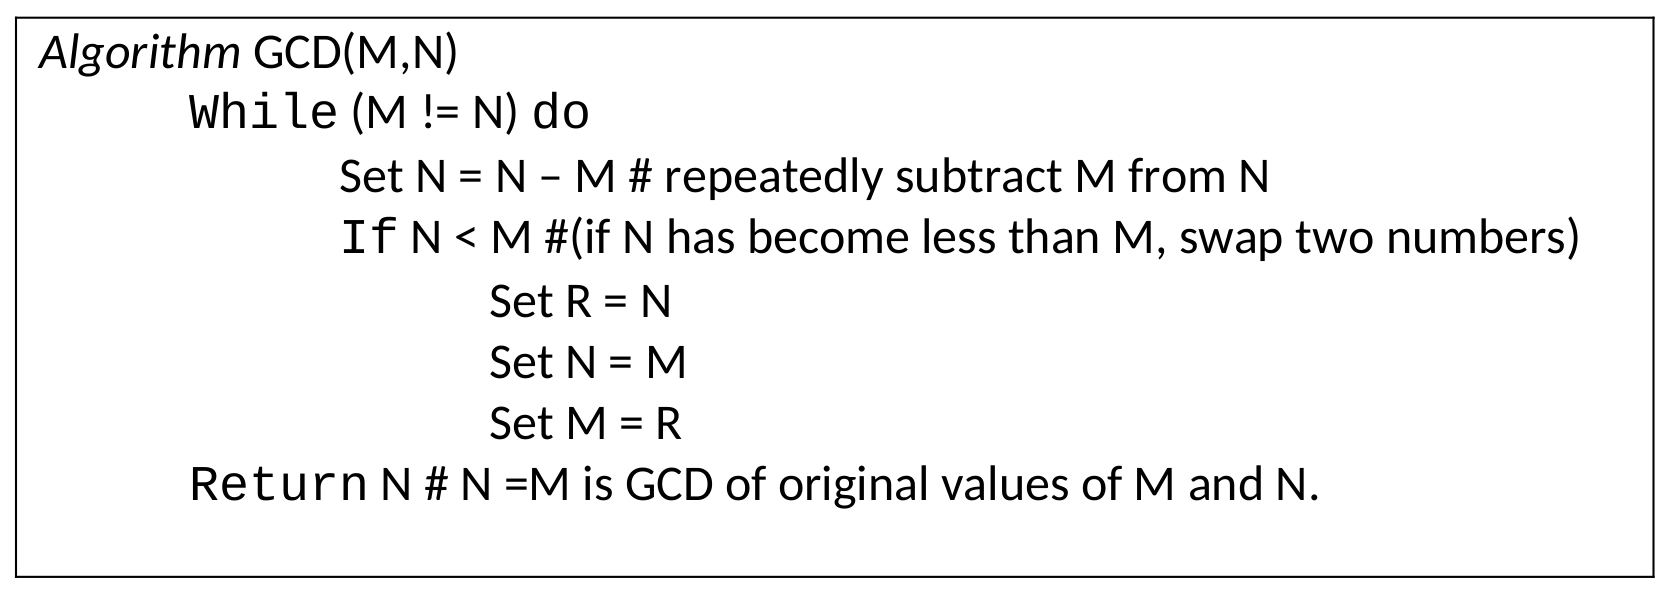
\includegraphics[scale=.65]{src/Figures/chap2/table5.jpg}
\end{table}


\begin{table}[H]

\vspace{-.3cm}

\centering
\caption{Algorithm for computing GCD using remainder}\label{chapter-3-table-6}
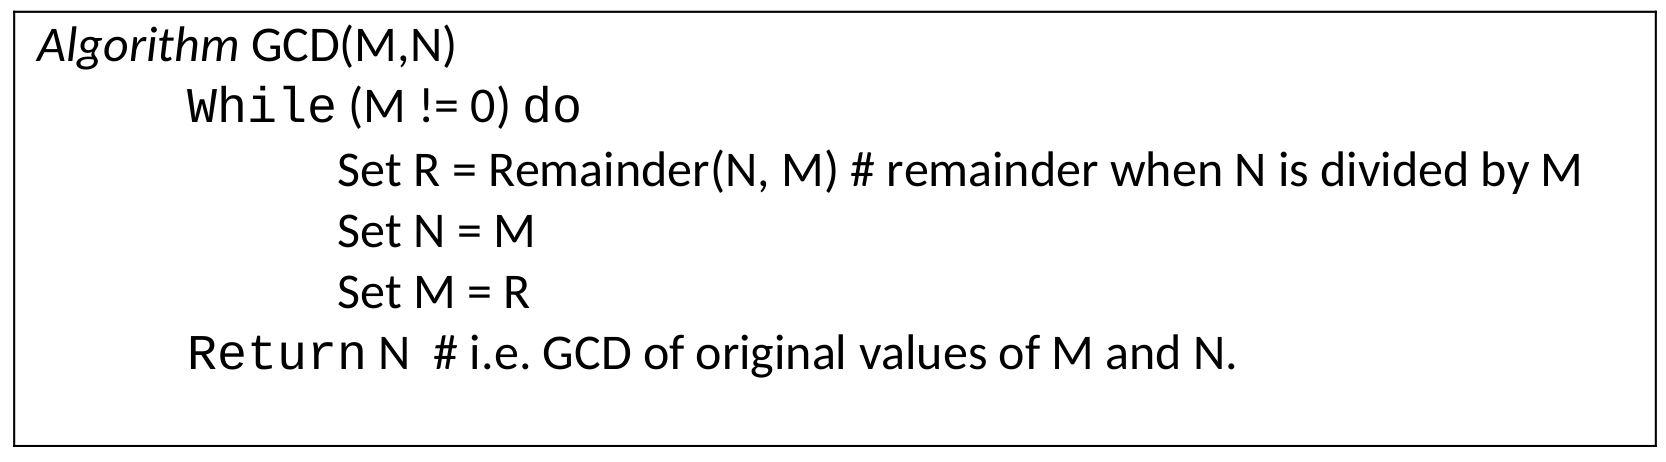
\includegraphics[scale=.65]{src/Figures/chap2/table6.jpg}
\end{table}

\hfill\raisebox{.3cm}{
\includegraphics[scale=.9]{src/Figures/circledC.eps}}

\vspace{-.3cm}


\begin{thebibliography}{99}

\bibitem{art2-key01} Aspiring Minds, ``National Employablity Report - Engineers Annual Report 2019", 

\url{https://www.aspiringminds.com/wp-content/uploads/2019/05/NER\_Engineer\_2019-V5}, last accessed March 2021.

\bibitem{art2-key02} Anany Levitin, ``Introduction to the Design and Analysis of Algorithms", 2$^{\rm nd}$ edition, Pearson Education.

\bibitem{art2-key03} Alexander Bogomolny, ``Interactive Mathematics Miscellany and Puzzles", 

\url{http://www.cut-the-knot.org/blue/EuclidAlg.shtml}, last acchessed March 2021.
 
\end{thebibliography}

\end{multicols}

\vskip -.2cm

\noindent
\begin{tabular}{V{2.5}cp{14.2cm}V{2.5}}
\clineB{1-2}{2.5}
 &\\
\raisebox{-4cm}{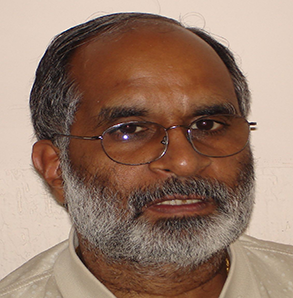
\includegraphics{src/Figures/authors/Rustagi_RPR-PP-Photo.png}} & 

\centerline{\large\bf Prof. Ram P. Rustagi}

\bigskip
Dr.~Ram P. Rustagi is currently working as Professor, CSE dept, KSIT Bangalore, and honed up his academic skills with Ph.D from IIT Delhi, and M.Tech from IISc Bangalore. Prior to KSIT, at Cavisson Systems, he mentored new technology development using Machine Learning techniques in Security and Performance Monitoring.~At PES University, he had taught Undergraduates, Post Graduates students, and successfully guided 3 Ph.D scholars. At PESU, he brought innovations in teaching computer network and security courses, and introduced practical experiential learning exercises.\\
&\\  
\raisebox{-3.7cm}{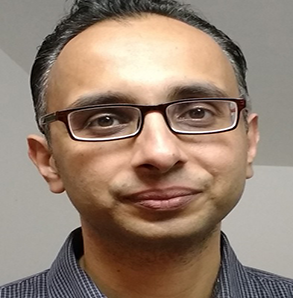
\includegraphics{src/Figures/authors/Viraj_Kumar.png}} & 

\centerline{\large\bf Prof. Viraj Kumar}

\bigskip
Dr.~Viraj Kumar is a Visiting Professor at the Divecha Centre for Climate Change, IISc Bangalore and the Vice-Chair of ACM India’s Special Interest Group in Computer Science Education (iSIGCSE). He was a consultant to the Committee to draft the National Education Policy (2017-18), and contributed to two education-related task groups of the Karnataka Knowledge Commission (2014-16). He holds a PhD in Computer Science from the University of Illinois at Urbana-Champaign.\\
&\\
\clineB{1-2}{2.5}
\end{tabular}

